%===============================================================================
% Advanced Thread Programming.
%===============================================================================

\section{Advanced Thread Programming}

\begin{itemize}
\item Quick Recapitulation of Threads
\item Other Existing Implementations of Threads
\item \texttt{fork()} and Threads
\item More on Thread Cancellation
\item MT-Level Attributes
\item Solaris Threads API
\item Threads and Performance
\end{itemize}

%\begin{itemize}
%\item ~
%\end{itemize}

%===============================================================================

\subsection{Very Quick Recap of Threads}


\begin{quote}
Multithreading is a programming and execution model that allows multiple threads
to co-exist within the context of a single process. All threads share the
process' resources but are able to execute independently. Threads provide
developers with a useful abstraction of concurrent execution.

% empty para
~

However, perhaps the most interesting application of the technology is when it
is applied to a single process to enable parallel execution of threads on a
multiprocessor system.
\end{quote}


\begin{itemize}
\item Great introduction to threads including some of the history around
this technology can be found in document ''Multithreading in the Solaris
Operating Environment''.
\end{itemize}

%===============================================================================

\subsection{Very Quick Recap of Threads (cont.)}

\begin{itemize}
\item main differences between a thread and a process
\item per thread attributes -- instruction counter, stack, thread ID, ...
\item when to use processes and when to use threads
\item type of implementations of threads
	\begin{itemize}
	\item user-level library (through \texttt{setjump}/\texttt{longjump}
	calls), inherently M:1
	\item kernel (1:1)
	\item hybrid (M:N)
	\end{itemize}
\end{itemize}

\begin{itemize}
\item M:1 means that multiple threads are mapped to one process only. Thus, the
kernel does not know about those threads at all, and in fact does not need to
support any kernel threads. If one thread blocks, the whole process would block
so a thread user-level library must replace blocking function calls with
non-blocking ones.
\item Hybrid M:N approach could be quite difficult to implement, you may be
mapping, say, 23 threads used by your application to 5 kernel threads. The idea
was to use as many threads as needed while not doing so many kernel switches
between those. However, you need two schedulers, for example -- one that
schedules the kernel threads, and one that schedules the user threads. Solaris
abandoned this approach, and NGPT (see page \pageref{NGPT}) was not chosen as
the replacement LinuxThreads library, see below. It seems that much simpler 1:1
approach is generaly the winning one.
\item The assumption that a kernel context switch must be inherently more
expensive than a thread context switch in user level might be tricky. You must
do a lot of things the same whether it is a switch in the kernel or in user
space, and the user space switch typically involves several system calls anyway
- you need to poll to see if the upcoming potentially blocking call is going to
block or not, and if it is then you need to save the current state and use a
long jump to switch to another thread. And there is more to it, see the
reference below.
\item Since FreeBSD 7, an alternative threading library there is
\texttt{libkse(3)} which is M:N. The default threading library is still 1:1
\texttt{libthr(3)} though.
\item References:
	\begin{itemize}
	\item See [\myun\myix-prog] for more information on thread basics.
	\item Very good discussion on M:N versus 1:1 mapping:
	\url{http://xiao-feng.blogspot.com/2008/08/thread-mapping-11-vs-mn.html}
	\end{itemize}
\end{itemize}

%===============================================================================

\subsection{What we know (from POSIX API)}


\begin{itemize}
\item actions we already know how to perform
	\begin{itemize}
	\item creating, destroying, joining, and terminating threads, and
	setting thread attributes when creating a thread
	\end{itemize}
\item synchronization primitives we know
	\begin{itemize}
	\item mutexes, conditional variables, read-write locks
	\item POSIX semaphores were not in [\myun\myix-prog] but it is just an
	analogy to SysV semaphores
	\item barriers
	\end{itemize}
\item what else then do we need to know?
\end{itemize}

\begin{itemize}
\item {}[\myun\myix-prog] went through almost everything from [posix-threads].
\item \label{THREAD_RECAP} \emsl{Exercise:} to get your hands dirty with
threads again, without use of any existing source code files write a simple
program that creates two threads. Each thread writes a ``Hello world''-like
message on stdout to prove that the thread was really created, and then returns.
The main thread waits on both threads to complete before it returns. Writing
that should take 2 minutes and 20 lines of code :-).
\end{itemize}

%===============================================================================

\subsection{Other Implementations}

\begin{itemize}
\item Solaris Threads
\item protothreads
	\begin{itemize}
	\item low-overhead approach, non-preemptable threads with no stack
	\item context is hold in global variables
	%\item provide sequential flow of control
	\end{itemize}
\item POSIX user-space library implementation in FreeBSD 3.0
\item GNU Portable Threads (pth API)
	\begin{itemize}
	\item highly portable user-space threading library (M:1) implementation
	\item can emulate POSIX Thread API as well
	\end{itemize}
\item C Threads API (Mach OS)
\item and many, many more...
\end{itemize}

\begin{itemize}
\item ``Non-preemtable'' in protothreads means that a context switch can take
place on blocking operations only (\texttt{read()}, for example). No stack means
no local variables. Protothreads are targeted at severely memory constrained
systems, such as small embedded systems or wireless sensor network nodes but its
use it not limited to just that.
\item LinuxThreads was a partial implementation of POSIX Threads that has since
been superseded by the Native POSIX Thread Library (NPTL). LinuxThreads had many
problems owed directly to its implementation; each thread had its own PID, for
example, which is a violation of the POSIX standard. NPTL is fully incorporated
in the GNU C library now.
\item Linux version 2.4 had no real kernel thread support.
\item \label{NGPT} GNU Pth and NPTL are two distinct implementations. NPTL makes
use of the Linux kernel threads. There was also NGPT M:N aproach intended to
replace LinuxThreads but eventually NPTL was chosen (BTW, it is 1:1). Read more
on history of Linux threads on the Onlamp link below.
\item User-space implementation of threads, or ``user threads'', not relying on
the system thread support and able to run on systems without such a support at
all, is sometimes called ``green threads''. This seems to have come from the
Java world:

\begin{quote}
\emph{When Java 1.0 first came out on Solaris, it did not use the native Solaris
library libthread.so to support threads. Instead it used runtime thread support
that had been written in Java for an earlier project code-named ``Green.'' That
threading library came to be known as ``green threads.''}
\end{quote}
\item References:
	\begin{itemize}
	\item \url{http://en.wikipedia.org/wiki/Thread\_(computer\_science)}
	\item \url{http://en.wikipedia.org/wiki/LinuxThreads}
	\item \url{http://en.wikipedia.org/wiki/Native\_POSIX\_Thread\_Library}
	\item \url{http://onlamp.com/onlamp/2002/11/07/linux\_threads.html}
	\item protothread implementation: \url{http://www.sics.se/~adam/pt}
	\end{itemize}
\end{itemize}

%===============================================================================

\subsection{Fork and Threads in POSIX}

\begin{itemize}
\item discussed to some extent already in [\myun\myix-prog]
\item \texttt{fork} duplicates only the calling thread in the child
	\begin{itemize}
	\item was not true on Solaris 9 or earlier with Solaris Threads
	\item it used the ``fork all'' semantics (\texttt{forkall(2)}), as
	opposed to the ``fork one''
	\end{itemize}
\item fork-one safety issues
	\begin{itemize}
	\item when \texttt{fork} is used, threads must be well behaved
	\item imagine a thread that does not call \texttt{fork} but holds a
	mutex
		\begin{itemize}
		\item the thread will not be duplicated, leaving the mutex
		locked for ever
		\item the child will probably dead-lock sooner or later
		\end{itemize}
	\end{itemize}
\end{itemize}

\begin{itemize}
\item Remember that a locked mutex may be unlocked only by the thread that
locked it before. That's the difference between a mutex and a binary
se\-ma\-pho\-re.
\item The class of problems that can happen on fork are in general called ``fork
safety issues''.
\end{itemize}

%===============================================================================

\subsection{Memory Leaks on \texttt{fork(2)}}

\begin{center}
% XXX convert to PDF
% 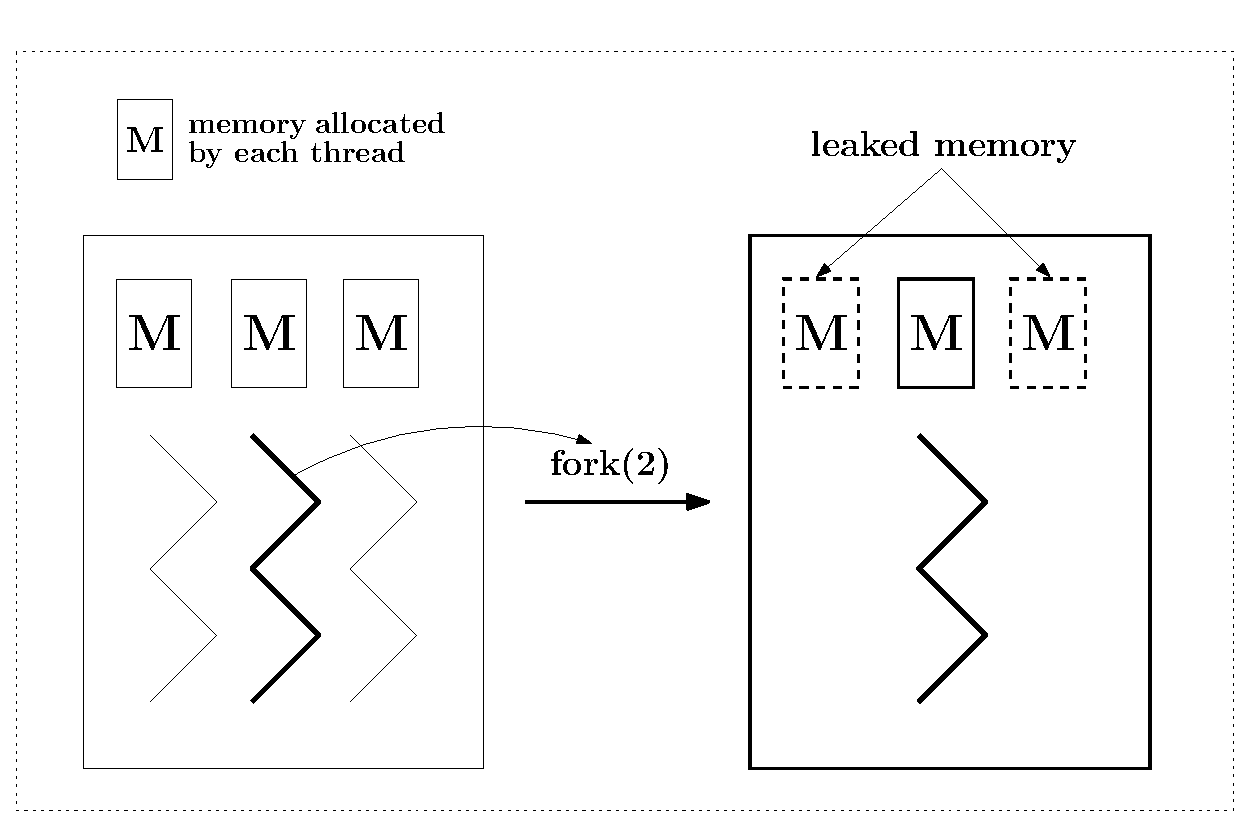
\includegraphics[width=100mm]{img/adv-thread-prog/mem-leaks-with-fork.eps}
\end{center}

\begin{itemize}
\item If a pointer to some memory dynamically allocated in each thread is on the
thread's stack only, such memory will be leaked if the thread is not the one
calling \texttt{fork(2)}. It happens in such a way because the thread, including
its stack, is not duplicated in the new process.
\end{itemize}

%===============================================================================

\subsection{Fork handlers - solution to fork-one safety issues}

\begin{verbatim}
int pthread_atfork(void (*prepare)(void),
                   void (*parent)(void),
                   void (*child)(void));
\end{verbatim}

\begin{itemize}
\item \texttt{prepare} is called before \texttt{fork} is started
\item \texttt{parent}/\texttt{child} are called in parent/child after
\texttt{fork}
\item \texttt{prepare} acquires all mutexes making sure no thread can hold any
lock
\item \texttt{parent}/\texttt{child} functions will release all locks after the
\texttt{fork} then
\end{itemize}

\begin{itemize}
\item Source: \texttt{adv-thread-prog/fork-one-issue.c} shows memory leaks in
the child, \texttt{adv-thread-prog/at\-fork.c} shows how to use the handlers in
general.
\item You may use fork handlers with a process with the \texttt{main()} thread
only, of course, which make them quite a general tool to use.
\item It is not just about mutexes and memory leaks. Imagine a library that has
some kernel state (ie. a handler to some kernel table slot):
	\begin{itemize}
	\item A \texttt{fork} will duplicate the user-level data.
	\item Kernel state will stay the same but now we have 2 processes with a
	handler to the same slot in a kernel table (which holds a reference
	counter equal to 1, not 2).
	\item When one process releases the handler the other thread one can no
	longer work with it since the reference counter dropped to 0, leading to
	the slot deallocation.
	\item For example, PKCS\#11 fork safety issues stem from the fact that
	according to the spec, the child should never use crypto sessions
	initialized in the parent.
		\begin{itemize}
		\item At-fork handlers can help here as well. The sessions are
		closed and initialized again (= the child will get its own
		kernel state structures) in the atfork functions.
		\end{itemize}
	\end{itemize}
\item \texttt{pthread\_atfork()} is not a necessary solution for
\texttt{fork-one-issue.c}. Given you cannot give any parameters to those
functions, global memory would have to be used to store all the pointers anyway
so that we could free those in the child. That means that (a) mdb would show no
memory leaks and (b) we could free all the pointers in the child after the fork.
However, we would have to do that manually which might not be possible -- we
could fork in a library function without knowing about it, for example.
\item In a threaded application, you usually need to fork only to run an
external command, either explicitly or implicitly through a library call. If you
need to do something else you create a new thread, not a new process, so those
problems with mutexes might seem quite unreal -- the external command can not
use those mutexes at all. However, the example above, about PKCS\#11, shows a
real example of a library that uses PKCS\#11 API, and an application that knows
nothing about it while forking a child. That's how SunSSH uses the OpenSSL
PKCS\#11 engine to offload crypto operations to the hardware accelerator. You
must be careful not to create a dead-lock in the library then.
\item Source: another example showing what happens if we hold a mutex in a
thread that has not called \texttt{fork},
\texttt{adv-thread-prog/mutex-with-atfork.c}.
\item \emsl{Exercise:} fix \texttt{adv-thread-prog/fork-one-issue.c} with the
fork handlers (ie. do not free the allocated memory in the child manually). Of
course that you will have to use global memory to store the memory pointers
anyway. Also remember that you should not free memory allocated in the thread
that called \texttt{fork(2)} -- it will probably need it.
\end{itemize}

%===============================================================================
\subsection{Fork-Safe Library}

Library can take care of the fork issues itself. On Solaris,
\texttt{attributes(5)} defines a \emph{Fork-Safe} library as the one that:

\begin{quote}
When \texttt{fork()} is called, a Fork-Safe library  arranges  to have  all  of
its internal locks held only by the thread performing the fork. This is usually
accomplished  with \texttt{pthread\_atfork(3c)},  which is called when the
library is initialized.
\end{quote}

...which is exactly what was discussed on the previous slide.

\begin{itemize}
\item ``Fork-Safe'' is actually one of the categories of the ``MT-Level''
attribute. More information is also on page \pageref{MT_LEVEL}. See
\texttt{at\-tr\-ibu\-tes(5)} for more information on attributes in general.
\end{itemize}
%===============================================================================

\subsection{More on thread cancellation}

\begin{itemize}
\item cancellation is good for situations where, for example:
	\begin{itemize}
	\item user is requesting to close or exit some running operation
	\item number of threads are solving a problem, one thread finds the
	solution, and all the remaining threads can be cancelled
	\end{itemize}
\item you must be careful
	\begin{itemize}
	\item calling a cancel-unsafe library might cause a problem in certain
	situations
	\begin{itemize}
		\item the thread might be cancelled while in a library call
		which might cause dead locks, memory leaks, etc.
		\end{itemize}
	\item \texttt{pthread\_setcancelstate()} can be called to temporarily
	disable cancellation
	\end{itemize}
\item \emph{cancellation point} is a place at which cancellation can occur
\end{itemize}


\begin{itemize}
\item Source code file \texttt{adv-thread-prog/pthread-cancel.c} borrowed from
[\myun\myix-prog] recaps how it works.
\item The specification names the list of calls that must function as
cancellation calls with another list of calls that may be cancellation points.
See the link below. The actual set is then defined by the system and not
suprisingly, each system documents it somewhere else. Solaris specifies the list
in the \texttt{cancellation(5)} man page, FreeBSD uses
\texttt{pthread\_cancel(3)}, Linux distros \texttt{pthreads(7)}.
\item References:
	\begin{itemize}
	\item Cancellation points are defined in the ``Thread Cancellation''
	section of
	\url{http://opengroup.org/onlinepubs/007908775/xsh/threads.html}
	\end{itemize}
\end{itemize}

%===============================================================================

\subsection{More on thread cancellation (cont.)}

\begin{itemize}
\item use \texttt{pthread\_testcancel()} to insert your own cancellation points
\item any call that might wait long should be a cancellation point
\item be careful with asynchronous cancellation
\item \texttt{pthread\_cleanup\_push()} should be used when a thread changes
some state and there is a possibility of cancellation
	\begin{itemize}
	\item the handler makes sure the state is reverted should there be any
	cancellation
	\item do not forget to pop the handler when the previously changed state
	has been restored
	\end{itemize}
\end{itemize}


\begin{itemize}
\item Asynchronous cancellation:
\begin{itemize}
\item Locked mutex in a cancelled thread can deadlock your application
or cause memory leaks.
\item In general, \emsl{the problem is to cancel a thread that holds some
resources}.
\end{itemize}
\item Cancel-Safe library pushes handlers wherever cancellation can occur, and
pops them when the state is restored. See \texttt{attributes(5)} man page on
Solaris.
\item \emsl{Exercise:} demonstrate a problem with a non-cancel-safe library.
Write a library with one function which internally uses dynamically allocated
memory. The memory is deallocated before the call returns. Use it the way that
\texttt{mdb} will report some memory leaks (sleep in the library before freeing
previously allocated memory and then cancel the thread from \texttt{main()}).
Then fix with \texttt{pthread\_cleanup\_push()} and a handler that deallocates
the memory should the thread be cancelled. Remember that shared library is
created using \texttt{--shared} option with \texttt{gcc} or \texttt{-G} with Sun
Studio (\texttt{cc}). Use \texttt{-R} and \texttt{-L} options properly.
\end{itemize}

%===============================================================================

\subsection{Cancel-Safety in Libraries}

On Solaris, \texttt{attributes(5)} defines a \emph{Cancel-\emsl{Unsafe}} library
as the one that:

\begin{quote}
If the thread has not installed the appropriate cancellation cleanup handlers to
release the resources appropriately (see \texttt{pthread\_cancel(3c)}), the
application is "cancel-unsafe", that is, it is not safe with respect to
cancellation.
\end{quote}

...and:

\begin{quote}
All applications that use \texttt{pthread\_cancel(3c)} should ensure that they
operate in a Cancel-Safe environment.
\end{quote}

There are two subcategories for libraries wrt cancel safety:
``Asynchronous-Cancel-Safety'' and ``Deferred-Cancel-Safe''.


\begin{itemize}
\item Obviously, Deferred-Cancel-Safety is easier to achieve than
Asynchronous-Cancel-Safety. \emsl{Most applications and libraries are expected
to always be Asynchronous-Cancel-Unsafe, unless explicitly specified otherwise.}
\end{itemize}

%===============================================================================

\subsection{MT-Level Attribute in General}

\label{MT_LEVEL}

In Solaris, there are more categories for the MT-Level attribute assigned to
libraries:

\begin{itemize}
\item \emph{Safe} -- can be used from multithreaded apps
\item \emph{Unsafe} -- library contains unprotected global and static data. Make
sure only 1 thread uses the library at a time
\item \emph{MT-Safe} -- fully prepared for multithreaded apps and should provide
reasonable concurrency
\item and some more
\end{itemize}

This is per function:

\begin{itemize}
\item \emph{Async-Signal-Safe} -- the function is MT-Safe and it can be safely
used from a signal handler
\end{itemize}

\begin{itemize}
\item Using a ``Safe'' library means that you will not dead-lock, crash or
corrupt its internal data if called from multiple threads. We can make an Unsafe
library a Safe one by surrounding an entire library with a mutex but such
aproach does not provide any concurrency. Thus, the library can be called Safe
but not MT-Safe.
\item Remember, using a function in a signal handler that is not ready for that
might result in a dead-lock. Imagine that another signal comes when the handler
is being already processed -- if the handler is used for that signal as well, we
can dead-lock if async-unsafe function is used. Note that 
\item In Solaris, every manual page for a function call has an
\texttt{ATTRIBUTES} section that also states a value of the MT-Level
attribute. Example from the \texttt{read(2)} manual page:

\begin{verbatim}
ATTRIBUTES
     See attributes(5) for descriptions of the following attri-
     butes:
     __________________________________________________________
    |       ATTRIBUTE TYPE      |       ATTRIBUTE VALUE       |
    |___________________________|_____________________________|
    | Interface Stability       | Committed                   |
    |___________________________|_____________________________|
    | MT-Level                  | read() is Async-Signal-Safe |
    |___________________________|_____________________________|
    | Standard                  | See standards(5).           |
    |___________________________|_____________________________|
\end{verbatim}
\end{itemize}

%===============================================================================

\subsection{Solaris Threads}

\begin{itemize}
\item in \texttt{libthread(3lib)} library shipped since Solaris 2.2 (1993)
	\begin{itemize}
	\item POSIX thread API not available at that time
	\item support for POSIX threads (pthreads) added in 2.5 (1995)
	\end{itemize}
\item Solaris API was also used in UNIX International spec
\item there are differences between both APIs
	\begin{itemize}
	\item but not major wrt functionality provided
	\end{itemize}
\item you can combine both APIs in one program
	\begin{itemize}
	\item note that the same kernel threads are underneath, API is just a
	way to work with those kernel threads
	\end{itemize}
\end{itemize}


\begin{itemize}
\item Basic information on the Solaris Threads API is in the
\texttt{libthread(3lib)} manual page on Solaris.
\item \label{THREAD_YIELD} Source: \texttt{adv-thread-prog/posix-with-yield.c}.
Read the opening comment for instructions on how to use the program.
\item Differences are listed in the \texttt{threads(5)} manual page. Look for
\texttt{THR\_DAEMON}, for example, that sounds interesting.
\item Both threading libraries were merged into \texttt{libc} since Solaris 10,
see the source code example.
\item References:
	\begin{itemize}
	\item UNIX International:
	\url{http://en.wikipedia.org/wiki/Unix\_International}
	\item Multithreading in the Solaris Operating Environment:
	See ``Reliable, Scalable Threads For All'' section for more information
        on the \texttt{libthread} library.
	\end{itemize}
\end{itemize}

%===============================================================================

\subsection{Solaris Threads API}

\begin{itemize}
\item no attribute objects as in POSIX threads -- you must use \texttt{flags}
\item use \texttt{<thread.h>} header file

\begin{verbatim}
int thr_create(void *stack_base, size_t stack_size,
               void *(*start_func) (void *), void *arg,
               long flags, thread_t *new_thread_ID);
\end{verbatim}

\item \texttt{start\_func} is the thread function
\item \texttt{arg} is the argument the function will be called with
\item you can use flags: \texttt{THR\_DETACHED}, \texttt{THR\_SUSPENDED} (the
thread is created suspended), \texttt{THR\_DAEMON} (the thread will continue to
operate after \texttt{main()} returned)
\end{itemize}


\begin{itemize}
\item As with \texttt{pthread\_create()}, the new thread inherits the signal
mask from the creating thread.
\item Default thread creation (\texttt{NULL} for the stack base and \texttt{0}
for the stack size makes the system use the default values) is like this:

\begin{verbatim}
thread_t tid;
void *start_func(void *), *arg;

thr_create(NULL, 0, start_func, arg, 0, &tid);
\end{verbatim}

It creates a joinable thread. The following piece of code creates a
detached thread:

\begin{verbatim}
thr_create(NULL, 0, start_func, arg, THR_DETACHED, NULL);
\end{verbatim}
\item \emsl{Exercise:} remember the simple recap program on threads on page
\pageref{THREAD_RECAP}? Rewrite it using Solaris Threads API. Note that joining
the thread is accomplished via \texttt{thr\_join()}, suprisingly.
\end{itemize}

%===============================================================================

\subsection{Differences between POSIX and Solaris Threads}

\begin{itemize}
\item POSIX threads can be cancelled
	\begin{itemize}
	\item this is a new thing introduced in POSIX threads
	\end{itemize}

\item Solaris threads can be suspended and resumed
	\begin{itemize}
	\item POSIX also does not have a yield (\texttt{thr\_yield()})
	\end{itemize}
\item in Solaris threads, we can wait for any thread
\item Solaris threads have no clean-up handlers for \texttt{fork(2)}
\item Solaris threads offer daemon threads
\item use POSIX threads on Solaris for new applications
	\begin{itemize}
	\item because that is the portable way of doing things
	\end{itemize}
\end{itemize}


\begin{itemize}
\item Waiting for any thread was intentionally not included in the POSIX
standard.
	\begin{itemize}
	\item There is no parent-parent relationship between threads.
	\item All threads aside from main are equal.
	\item So, there is no concept of ``waiting for a child thread'' as is in
	the pro\-cess environment.
	\end{itemize}
\item In Solaris threads, waiting for any thread is possible if 0 is used as the
thread ID:

\begin{verbatim}
if (thr_join(0, NULL, NULL) == 0) {
        ...
}
\end{verbatim}
\item In pthreads, you could easily simulate that using one thread (the main
one, perhaps) for waiting on a conditional variable while each finishing thread
would signal the variable right before returning from its function. Main could
then join the thread, getting its id from a protected global variable, for
example.
\end{itemize}

%===============================================================================

\subsection{Combining both APIs}

\begin{itemize}
\item works because those APIs "just" work with the same kernel entity -- the
thread
\item probably does not have much sense
\item maybe "fixing" old code with mechanisms provided in other thread API
	\begin{itemize}
	\item anyway, note that thread types are different - we cannot join
	POSIX thread with Solaris thread API call
	\end{itemize}
\end{itemize}

\begin{itemize}
\item Source: while we alread showed on page \pageref{THREAD_YIELD} that we can
yield threads created with POSIX API, the following program even creates threads
using both APIs: \texttt{adv-thread-prog/both-thread-APIs.c}.
\end{itemize}

%===============================================================================

\subsection{Threads and Performance}

\begin{itemize}
\item parallelism is one of the answers for a need to get higher performance
\item great for threads
\item however, threads bring inherent data sharing between them
\item need to synchronize
\item synchronization points, a shared structure for example, are candidates for
bottlenecks in the program performance
\item also, not everything is possible to parallelize -- CBC (cipher block
chaining) is one example
\end{itemize}

\begin{itemize}
\item On the wake of more and more multi-core CPUs emerging \emsl{it is always
important to realize what we can expect there}. In general, if you do not know
what to expect, you can not estimate various attributes of the project. If you
can not estimate, you can not manage the project.
\item With multiple cores, we can roughly expect linear increase in computation
power, depending on the system, program, and the type of a problem being solved,
of course. What's more, some cores are able to run more threads in parallel,
without a need for a software context switch. Thus, such threads can represent
something called \emph{virtual CPUs}. This idea in general is called \emph{Chip
Multi-Processing}.
\item One example of a CMP machine is UltraSPARC T1 or T2. T2 can have up to 8
cores with each core running up to 8 threads. T2 with 8 cores then have 64
virtual CPUs. However, how does that scale then? Take \texttt{u-us} in Mal\'a
Strana's lab. It's an UltraSPARC T1 machine with 6 cores (T1 can run up to 4
threads per core). So, \texttt{/usr/sbin/psrinfo} will show you 24 virtual CPUs.
With a simple program that runs just looping threads, we can see that we can get
70\% of the theoretical maximum and we even scale linearly up to 6 threads:

\begin{verbatim}
# We get 600% of a single thread performance if running with 6
# threads:
/a.out 6 10
1661374469
$ ./a.out 1 10
277845608
$ bc
6 * 277845608
1667073648

# With 24 threads we can see that virtual CPUs are not fully
# independent and that we get "only" 70% of the theoretical
# maximum:
$ ./a.out -g 24 10
Using global memory for counters.
4679205463
./a.out 1 10
277776481
$ bc
24 * 277776481
6666635544
scale=2
4679205463/6666635544
.70
\end{verbatim}
\item Source: \texttt{adv-thread-prog/parallel-computation.c}.
\end{itemize}

\endinput
